\documentclass[11pt,letterpaper]{article}
\usepackage{times}
\usepackage[onehalfspacing]{setspace}
\usepackage{natbib}\bibpunct{(}{)}{,}{}{}{,}
\usepackage{amsmath,amsfonts,amsthm}
\usepackage{comment}
\usepackage{tabularx}
\usepackage{multirow}
\usepackage{booktabs}
\usepackage{subcaption}
\usepackage{graphicx}
\usepackage[colorlinks,linkcolor=blue,citecolor=black,urlcolor=black]{hyperref}
\usepackage[title,titletoc]{appendix}
\usepackage{enumitem}
\usepackage{subcaption}  % For subfigures
\usepackage{lscape}      % For landscape orientation if needed
\usepackage[noabbrev,capitalize]{cleveref}
\usepackage{tikz}
\usetikzlibrary{shapes.geometric}
\usepackage{pgfplots}
\usetikzlibrary{patterns, pgfplots.fillbetween}
\usepackage{graphicx}
\usepackage{mathpazo}

% commands
\newtheorem{definition}{Definition}
\newtheorem{proposition}{Proposition}
\newtheorem{lemma}{Lemma}
\newcommand{\figpath}{fig/}
\newcommand{\tablepath}{table/}
\newcommand{\rmdi}{\mathrm{d}}

% table and figure formatting
%\input{formats}

% page size
\setlength{\textwidth}{\paperwidth}
\addtolength{\textwidth}{-1.7in}
\setlength{\oddsidemargin}{.85in}
\addtolength{\oddsidemargin}{-.85in}
\setlength{\evensidemargin}{\oddsidemargin}
\setlength{\headheight}{0pt}
\setlength{\headsep}{0pt}
\setlength{\textheight}{\paperheight}
\addtolength{\textheight}{-\headheight}
\addtolength{\textheight}{-\headsep}
\addtolength{\textheight}{-\footskip}
\addtolength{\textheight}{-1.75in}
\setlength{\topmargin}{1in}
\addtolength{\topmargin}{-1in}

\begin{document}

\title{\textbf{Specific Factors Model}}
\author{\large%
\setcounter{footnote}{0}%
Carlos G\'{o}es \\[-3pt] \textit{\small IFC, World Bank Group}
}
\maketitle

\paragraph{Production} Consider a world with 2 countries $i \in \{ H, F\}$ and two industries: agriculture $A$ and manufacturing $M$. In country $i$, there are $\bar{L}_i$ units of labor (worker-hours) available, which we call the labor endowment. There are also $\bar{T}_i$ hectares of land available as well as a fixed stock of capital denoted by $\bar{K}_i$.

In country $i$, firms producing good $g \in \{ A,M\}$ have a Cobb-Douglas technology satisfying:

\begin{equation*}
 Y_{i,M} = Z_{i,M} \times K_{i}^{\beta_i} L_{i,M}^{1-\beta_i}, \qquad  Y_{i,A} = Z_{i,A} \times T_{i}^{\beta_i} L_{i,A}^{1-\beta_i}
\end{equation*}

\noindent where the parameters $\{ Z_{i,M}, Z_{i,A}\}$ denote the total factor productivity of each sector in country $i$.

Here, land $T_i$ is a factor that is specific to the agricultural sector while capital $K_i$ is a factor that is specific to the manufacturing sector. This means that each sector is the exclusive user of that particular factor in country $i$ and in equilibrium they will use the whole available stock of that factor in the country (with adjusting to make sure supply equals demand).

Conversely, labor is a common and mobile factor. This means that, after some change in relative prices (or to some fundamentals that alter the marginal product of any of the factors), labor will to move across sectors to optimize the level of production and consumption. Labor allocations must satisfy:

\begin{equation*}
    L_{i,A} + L_{i,M} \le \bar{L}_i
\end{equation*}

\noindent i.e., the sum of the labor used in agriculture and manufacturing cannot be larger than the total labor endowment in the country.

Firms take factor prices as given and maximize profits under perfect competition:
        \begin{eqnarray*}\label{eq: production}
            &\max_{L_{i,M}, K_{i}}& P_{M} \times  Z_{i,M} \times K_{i}^{\beta_i} L_{i,M}^{1-\beta_i} - w_i L_{i,M} - r_{i,M} K_{i} \\
            &\max_{L_{i,A}, T_{i}}& P_{A} \times  Z_{i,A} \times T_{i}^{\beta_i} L_{i,A}^{1-\beta_i} - w_i L_{i,A} - r_{i,A} T_{i} 
        \end{eqnarray*}

This is a simple unconstrained maximization problem that you can solve by taking a derivative of the objective function with respect to each choice variable and setting it equal to zero. The optimal choices satisfy the marginal product of each factor (converted to dollars) being equal to their factor prices (why?):

\begin{eqnarray*}
    P_{M} \times  Z_{i,M} \times (1-\beta_i) \times \left( \frac{K_{i}}{L_{i,M}} \right)^{\beta_i} = P_M \times MPL_{i,M} &=& w_i \\
    P_{M} \times  Z_{i,M} \times \beta_i \times \left( \frac{L_{i,M}}{K_{i}} \right)^{1-\beta_i} = P_M \times MPK_{i,M} &=& r_{i,M} \\
    P_{A} \times  Z_{i,A} \times (1-\beta_i) \times \left( \frac{T_{i}}{L_{i,A}} \right)^{\beta_i} = P_A \times MPL_{i,A} &=& w_i \\
    P_{A} \times  Z_{i,A} \times \beta_i \times \left( \frac{L_{i,A}}{T_{i}} \right)^{1-\beta_i} = P_A \times MPT_{i,A} &=& r_{i,A}
\end{eqnarray*}

Note that, by combining the two optimality conditions with respect to labor, we can the derive the following relationship:

\begin{equation}\label{eq: mpl-prices}
    -\frac{MPL_{i,M}}{MPL_{i,A}} = \frac{\partial Y_{i,M}/\partial L_{i,M}}{\partial Y_{i,A}/\partial L_{i,A}} = MRT_{i,MA} = -\frac{P_A}{P_M}
\end{equation}
The left side of equation \eqref{eq: mpl-prices} is the slope of the production possibility frontier at the actual production point; the right side is minus the relative price of manufactures. This result tells us that at the production point, the production possibility frontier must be tangent to a line whose slope is minus the price of agriculture divided by that of manufactures. That ratio is also equal to the ``marginal rate of transformation'' -- i.e., how many extra units of $M$ society gets by forgoing one unit of $A$. We will come back to this point later. 


\newpage

\begin{figure}[htp]
    \centering
    \begin{tikzpicture}
    \begin{axis}[
        axis lines=middle,
        xmin=-1.25, xmax=1.25,
        ymin=-1.25, ymax=1.25,
    %    xlabel={\small Output of cloth / Labor in cloth},
    %    ylabel={\small Output of food / Labor in food},
        xtick=\empty,
        ytick=\empty,
        axis line style={<->},
        clip=false,
        enlargelimits=false,
        domain=0.0:1,
        width=0.75\textwidth,
        height=0.75\textwidth,
        samples=200
    ]
    
    \pgfmathsetmacro{\a}{0.5}       % curvature parameter
    
    % NW: Production function for food (plot in 2nd quadrant)
    \addplot[black, thick] ({-x}, {x^(\a)});
    \node[anchor=east] at (axis cs:-1.25,0) {\scriptsize $L_{i,M}$};
    \node[anchor=south] at (axis cs:0,1.25) {\scriptsize $Y_{i,M}$};
    
    % SW: Labor allocation AA curve (line in 3rd quadrant)
    \addplot[brown, thick] ({-x}, {-1 + x});
    %\node[anchor=north east] at (axis cs:-0.95,-0.05) {\scriptsize Economy's allocation of labor (AA)};
    
    % SE: Production function for cloth (4th quadrant)
    \addplot[blue, thick] ({x^(\a)}, {-x});
    \node[anchor=west] at (axis cs:1.25,0) {\scriptsize $Y_{i,A}$};
    \node[anchor=north] at (axis cs:0,-1.25) {\scriptsize $L_{i,A}$};
    %\node[anchor=north west] at (axis cs:0.6,-0.6) {\scriptsize Production function for cloth};
    
    % NE: Production Possibility Frontier (PPF)
    \addplot[red, thick] ({x^(\a)}, {(1 - x)^(\a)});
    %\node[anchor=south east, blue] at (axis cs:0.6,0.65) {\scriptsize $PP$};
    
    % point on AA
    \addplot+[mark=*,only marks,mark size=1.5pt,brown]
                  coordinates {({-0.5},{-1+0.5})}
                  node[anchor=north east,font=\scriptsize, brown] {$(L_{i,M}^*,L_{i,A}^*)$};
    
    \addplot[dashed, gray] coordinates {({-0.5}, {-1 + 0.5}) (0, {-1 + 0.5})};

    \addplot+[mark=*,only marks,mark size=1.5pt,black]
                  coordinates {({-0.5}, 0)}
                  node[anchor=north east,font=\scriptsize] {$L_{i,M}^*$};

        \addplot+[mark=*,only marks,mark size=1.5pt,black]
                  coordinates {(0, {0.5^(\a)})}
                  node[anchor=south east,font=\scriptsize] {$Y_{i,M}^*$};

    % Project to NW (Food PF)
    \addplot[dashed, gray] coordinates {({-0.5}, 0) ({-0.5}, {0.5^(\a)})};
    \addplot[dashed, gray] coordinates {(0, {0.5^(\a)}) ({-0.5},{0.5^(\a)})};
    \addplot+[mark=*, only marks, mark size=1.5pt, black]
            coordinates {({-0.5}, {0.5^(\a)})}
            node[anchor=north east, font=\scriptsize]{$(L_{i,M}^*,Y_{i,M}^*)$};     

    \addplot[dashed, gray] coordinates {({-0.5}, 0) ({-0.5}, {-(1-0.5)})};
    \addplot+[mark=*,only marks,mark size=1.5pt,black]
                  coordinates { (0, {-(1-0.5)})}
                  node[anchor=north east,font=\scriptsize] {$L_{i,A}^*$};

        % Project to SE (Cloth PF)
    \addplot[dashed, gray] coordinates {(0, {-0.5}) ({0.5^(\a)}, {-0.5})};
    \addplot[dashed, gray] coordinates {({0.5^(\a)}, 0) ({0.5^(\a)}, {-0.5})};
    \addplot+[mark=*, only marks, mark size=1.5pt, black]
            coordinates {({0.5^(\a)}, {-0.5})}
            node[anchor=south west,font=\scriptsize] {$(Y_{i,A}^*,L_{i,A}^*)$};
    
    \addplot+[mark=*,only marks,mark size=1.5pt,black]
                  coordinates { (0, {-(1-0.5)})}
                  node[anchor=north east,font=\scriptsize] {$L_{i,A}^*$};

        \addplot+[mark=*,only marks,mark size=1.5pt,black]
                  coordinates {({0.5^(\a)},0)}
                  node[anchor=south west,font=\scriptsize] {$Y_{i,A}^*$};


    % Project to NE (PPF)
    \pgfmathsetmacro{\Qc}{0.5^(\a)}
    \pgfmathsetmacro{\Qf}{(1 - 0.5)^(\a)}
    \addplot+[mark=*, only marks, mark size=1.5pt]
            coordinates {(\Qc, \Qf)}
            node[anchor=south west, font=\scriptsize, black]{$Y_{i,A}^*,(Y_{i,M}^*)$};     
    \addplot[dashed, gray] coordinates {(\Qc, 0) (\Qc, \Qf)};
    \addplot[dashed, gray] coordinates {(0, \Qf) (\Qc, \Qf)};
    \addplot[dashed, gray] coordinates {(0, \Qf) (\Qc, \Qf)};

    
    \end{axis}
    
    \end{tikzpicture}
    
    \caption{Allocation in this economy. \textcolor{brown}{Southwest: labor endowment constraint, the maximum allocation choices of labor $\bar{L}_i = L_{i,A} + L_{i,M}$}; \textcolor{blue}{Southeast: production function for agriculture as a function of labor input $Y_{i,A} = Z_{i,A} T_{i}^{\beta_i} L_{i,A}^{1-\beta_i}$}; \textcolor{black}{Northwest: production function for manufacturing as a function of labor input $Y_{i,M} = Z_{i,M} K_{i}^{\beta_i} L_{i,M}^{1-\beta_i}$}; \textcolor{red}{Northeast: production possibilities frontier $Y_{i} = Y_{i,A} + Y_{i,M}$.}}
    \label{fig:enter-label}
\end{figure}

\paragraph{Demand} Households in each country $i$ have three sources of income: (a) they supply their time time for wage $w_i$ and earn labor income $w_i L_i$; (b) they rent their land to agricultural producers and earn income $r_{i,A} T_{i}$; and (c) they rent their capital to manufacturing producers and earn income $r_{i,M} K_{i}$. They have preferences over the consumption of goods $p \in \{ A, M\}$, purchase quantities $Q_{i,A}, Q_{i,M}$ for prices $P_{A}, P_{M}$ and exhaust their income, maximizing:

\begin{equation*}
    \max_{\{Q_{i,A}, Q_{i,M}\}} U_i(Q_{i,A}, Q_{i,M}) \equiv Q_{i,A}^{\alpha_i} Q_{i,M}^{1-\alpha_i} \qquad s.t. \qquad P_{A} Q_{i,A} + P_{M} Q_{i,M} = I_i = w_i \bar{L}_i + r_{i,A} T_{i} + r_{i,M} K_{i}
\end{equation*}

This is a simple constrained concave maximization problem, that you should know how to solve from your calculus classes. One way to solve it is to replace the constraint into the objective function. Note $Q_{i,M} = \frac{I_i}{P_{M}} - \frac{P_{A}}{P_{M} } Q_{i,A}$, so the maximization problem below is equivalent to the original one:

\begin{equation*}
    \max_{\{Q_{i,A}\}} U_i(Q_{i,A}, Q_{i,M}(Q_{i,A})) \equiv Q_{i,A}^{\alpha_i} \left( \frac{I_i}{P_{M}} - \frac{P_{A}}{P_{M} } Q_{i,A} \right)^{1-\alpha_i}
\end{equation*}

\noindent for which we can take a derivative and set it equal to zero to find the optimal point:

\scriptsize{
\begin{eqnarray*}
    & & \alpha_i Q_{i,A}^{\alpha_i-1} \left( \underbrace{\frac{I_i}{P_{M}} - \frac{P_{A}}{P_{M} } Q_{i,A}}_{=Q_{i,M}} \right)^{1-\alpha_i} + Q_{i,A}^{\alpha_i} (1-\alpha_i) \left( \underbrace{\frac{I_i}{P_{M}} - \frac{P_{A}}{P_{M} } Q_{i,A}}_{=Q_{i,M}} \right)^{1-\alpha_i-1} \left( - \frac{P_{A}}{P_{M}}\right) = 0 \\
%    & & \alpha_i  \left( \frac{Q_{i,M}}{Q_{i,A}} \right)^{1-\alpha_i} - (1-\alpha_i) \left( \frac{Q_{i,M}}{Q_{i,A}} \right)^{-\alpha_i} \left( \frac{P_{A}}{P_{M}}\right) = 0 \\
%    & & \alpha_i  \left( \frac{Q_{i,M}}{Q_{i,A}} \right)^{1-\alpha_i} = (1-\alpha_i) \left( \frac{Q_{i,M}}{Q_{i,A}} \right)^{-\alpha_i} \left( \frac{P_{A}}{P_{M}}\right) \\
%    & & \frac{Q_{i,M}}{Q_{i,A}}  = \frac{1-\alpha_i}{\alpha_i } \left( \frac{P_{A}}{P_{M}}\right) \\
\iff    & & Q_{i,M}  = \frac{1-\alpha_i}{\alpha_i } \left( \frac{P_{A}}{P_{M}}\right) Q_{i,A}
\end{eqnarray*}
}

\normalsize
Replacing the last line into the budget constraint:

\scriptsize{
\begin{eqnarray*}
    Q_{i,M}&=& \frac{I_i}{P_{M}} - \frac{P_{A}}{P_{M} } Q_{i,A} \\
    \frac{1-\alpha_i}{\alpha_i } \left( \frac{P_{A}}{P_{M}}\right) Q_{i,A} &=& \frac{I_i}{P_{M}} - \frac{P_{A}}{P_{M} } Q_{i,A} \\
%    \frac{1-\alpha_i}{\alpha_i } \left( \frac{P_{A}}{P_{M}}\right) Q_{i,A} + \frac{P_{A}}{P_{M} } Q_{i,A} &=& \frac{w_i L_i}{P_{M}}  \\
%    \frac{1-\alpha_i + \alpha_i}{\alpha_i } \left( \frac{P_{A}}{P_{M}}\right) Q_{i,A} &=& \frac{w_i L_i}{P_{M}}  \\
    Q_{i,A} &=& \alpha_i  \frac{I_i}{P_{A}}
\end{eqnarray*}

}

\normalsize
Finally:
{\scriptsize
\begin{eqnarray*}
     Q_{i,M}  &=& \frac{1-\alpha_i}{\alpha_i } \left( \frac{P_{A}}{P_{M}}\right) Q_{i,A}  \\
     Q_{i,M}  &=& \frac{1-\alpha_i}{\alpha_i } \left( \frac{P_{A}}{P_{M}}\right) \alpha_i  \frac{I_i}{P_{A}} \\
      Q_{i,M}  &=& (1-\alpha_i) \frac{I_i}{P_{M}}
\end{eqnarray*}
}
\normalsize
Therefore, optimal demand functions satisfy:

\begin{equation}\label{eq: demand}
    Q_{i,A} = \alpha_i  \frac{I_i}{P_{A}}, \qquad Q_{i,M} = (1-\alpha_i) \frac{I_i}{P_{M}}
\end{equation}
\normalsize

Under Cobb-Douglas preferences, each consumer allocates a fixed share of their income—determined by their preference parameter $(\alpha_i, 1-\alpha_i)$ to each good, purchasing quantities inversely proportional to the price of that good. This holds regardless of whether consumers are in autarky or trade.

From equation \eqref{eq: mpl-prices}, we know relative prices are equal to the ratio of marginal products. From the demand functions, we can derive the marginal rate of substitution:

\begin{equation}
    -MRS_{i,AM} = -\frac{\partial U_i / \partial Q_{i,A} }{ \partial U_i / \partial Q_{i,M} } = -\frac{\alpha_i}{1-\alpha_i} \frac{Q_{i,M}}{Q_{i,A}} = -\frac{P_A}{P_M} = MRT_{i,MA}
\end{equation}

Therefore, as we see in Figure \eqref{fig: consumption} below, the equilibrium choice of consumption will be where the indifference curve is tangent to the price line. In autarky, that is also happens to be the tangent point of the PPF, as stated by equation \eqref{eq: mpl-prices}.


\newpage


\begin{figure}
    \centering
    \begin{tikzpicture}
    \pgfmathsetmacro{\alpha}{0.5}    % preference for computers
    \pgfmathsetmacro{\beta}{0.5}    % preference for computers

    \pgfmathsetmacro{\Zm}{1}
    \pgfmathsetmacro{\K}{1}
    
    \pgfmathsetmacro{\Za}{1}
    \pgfmathsetmacro{\T}{1}

    \pgfmathsetmacro{\L}{1}

    \pgfmathsetmacro{\P}{ \Za / \Zm * ((1-\alpha)/\alpha * \T / \K )^(\beta)  }
    
    \pgfmathsetmacro{\Omega}{(\P *\Zm / \Za)^(1/\beta) * \K / \T}      
    \pgfmathsetmacro{\Ls}{ \Omega / (1+\Omega) * \L}
    
    \pgfmathsetmacro{\Ym}{ \Zm * \K^(\beta) * \Ls^(1-\beta) }
    \pgfmathsetmacro{\Ya}{ \Za * \T^(\beta) * (1-\Ls)^(1-\beta) }

%    \pgfmathsetmacro{\ws}{ \Pm * \Zm * (1-\beta) * (\K / \Ls )^(\beta) }   
    % Compute utility level
    \pgfmathsetmacro{\U}{(\Ya^(\alpha))*(\Ym^(1 - \alpha))}
    
    % Compute prefactor for indifference curve: Qc = A * Qr^(- (1 - alpha)/alpha)
    \pgfmathsetmacro{\expo}{(1 - \alpha)/\alpha}
    \pgfmathsetmacro{\A}{\U^(1/\alpha)}
    
    \centering
    \begin{axis}[
        xlabel={Quantity of manufacturing, $\textcolor{red}{Q_{i,M}}, \textcolor{blue}{Y_{i,M}}$},
        ylabel={Quantity of food, $\textcolor{red}{Q_{i,A}}, \textcolor{blue}{Y_{i,A}}$},
        ymin=0, ymax=\L+.5,
        xmin=0, xmax=\L+.5,
        yticklabel=\empty,
        xticklabel=\empty,
        axis lines=left,
        enlargelimits=false,
        clip=false,
        axis on top,
        scaled x ticks=false,
        width=9cm, height=7cm,
        title style={font=\bfseries}
    ]
    
    % PPF: Q_C = (L/a_C) - (a_R/a_C) * Q_R
    \addplot[blue, thick, domain=0:1] ({ \Zm * \K^(\beta) * (\L-x)^(1-\beta)}, {\Za * \T^(\beta) * (x)^(1-\beta)});
    \pgfmathsetmacro{\c}{ \Ym + \P * \Ya }
    \addplot[thick, brown, domain=0.2:1.2] { \c - \P*x};
    
    % Indifference curve through optimal bundle
    \addplot[thick, red, domain=0.3:1.2, samples=100] {\A * x^(-\expo)};
    
    % Labels
    %\node at (axis cs:3.5,0.03) {\Large $\mathcal{Y}_{US}$};
    %\node at (axis cs:\Lendow/\aR,-.01) {\scriptsize $\frac{L_{US}}{a_{US,R}}$};
    %\node at (axis cs:-.75,\Lendow/\aC) {\scriptsize $\frac{L_{US}}{a_{US,C}}$};
    
    
    % Equilibrium point
    \addplot[only marks, mark=*, color=black, mark size=2pt] coordinates {(\Ym, \Ya)};
    \addplot[dashed] coordinates {(\Ym,\Ya) (\Ym,\Ya-.2)};
    \addplot[dashed] coordinates {(\Ym,\Ya-.2) (\Ym+\P*.2,\Ya-.2)};
    \node at (axis cs:\Ym + .15,\Ya + 0.1) {\scriptsize $(Q_{i,M},Q_{i,A})$};
    \node at (axis cs:\Ym+ .1,\Ya-.25) {\scriptsize $1$};
    \node at (axis cs:\Ym- .05,\Ya-.1) {\scriptsize $\frac{P_M}{P_A}$};
    %\node at (axis cs:\Qr - 2,\Qc + 0.0025) {\scriptsize $\textcolor{blue}{(Y_{US,R},Y_{US,C})}$};
    
    
    
    \end{axis}
    \end{tikzpicture}
    
    \caption{Optimal Consumption and Production Choices}
    \label{fig: consumption}
\end{figure}


\paragraph{Labor Market Equilibrium} Since households supply labor inelastically, then total labor supply will be equal to the total labor endowment and $\bar{L}_i = L_{i,A} + L_{i,M}$. The same is true for capital demand $K_i = \bar{K}_i$ and land demand $T_i = \bar{T}_i$. As a consequence:

\begin{equation} \label{eq: l-constraint}
    L_{i,A} + L_{i,M} = \bar{L}_i \iff L_{i,A} =  \bar{L}_i -  L_{i,M}
\end{equation}

Note that, from the first order conditions of the firms:

\begin{equation} \label{eq: equal-wage}
   P_M \times MPL_{i,M} = w_i = P_A \times MPL_{i,A}
\end{equation}

In English, the condition above means that labor demand will shift across sectors up to the point in which the marginal cost of hiring one extra worker (the wage $w_i$) is exactly the same as the marginal revenue that such an extra worker brings to the firm ($P_M \times MPL_{i,M}$ in manufacturing or $P_A \times MPL_{i,A}$ in agriculture).

If the wage is higher than the marginal revenue, the firm can decrease its losses by firing an extra worker (decrease its labor demand). If the wage is lower than the marginal revenue, the firm can make a higher profit by hiring an extra worker (increase its labor demand). This dynamic would play out until the firm hires the just right number of workers and the marginal cost of hiring an extra worker equals the marginal revenue that worker brings in. We plot that intuition in Figure \ref{fig: mpl}.

\begin{figure}
    \centering
        \begin{tikzpicture}
        
        \pgfmathsetmacro{\alpha}{0.5}    % preference for computers
        \pgfmathsetmacro{\K}{1}    % labor endowment
        \pgfmathsetmacro{\A}{1}    % labor endowment
        
        \centering
        \begin{axis}[
            ylabel={$\textcolor{red}{P \times MPL}$, $w$ },
            xlabel={Used labor input: $L$},
            ymin=0, ymax=1.5,
            xmin=0, xmax=5,
            yticklabel=\empty,
            xticklabel=\empty,
            axis lines=left,
            enlargelimits=false,
            clip=false,
            axis on top,
            scaled x ticks=false,
            width=9cm, height=7cm,
            title style={font=\bfseries}
        ]
        
        % PPF: Q_C = (L/a_C) - (a_R/a_C) * Q_R
        \addplot[thick, red, domain=0:5] {(1-\alpha)*\A*\K^(\alpha)/x^(\alpha)};
        
        
        \addplot[dashed, purple, ->] coordinates {(0.5  , {(1-\alpha)*\A*\K^(\alpha)/0.5^(\alpha)}) (0.5 + 0.3, {(1-\alpha)*\A*\K^(\alpha)/0.5^(\alpha)} + 0.2)};
        \addplot[mark=*, only marks, purple, mark size=1pt] coordinates {(0.5, {(1-\alpha)*\A*\K^(\alpha)/0.5^(\alpha)})};
        \node[anchor=south west, purple] at (axis cs:0.5 + 0.3, {(1-\alpha)*\A*\K^(\alpha)/0.5^(\alpha)} + 0.25) {\scriptsize $P\times MPL > w^*$: hired too little};
        
        \pgfmathsetmacro{\Lb}{((1-\alpha)* \A / 0.5)^(1/\alpha) * \K}    % labor endowment
        
        \addplot[dashed, blue, ->] coordinates {(\Lb, {(1-\alpha)*\A*\K^(\alpha)/\Lb^(\alpha)}) (\Lb + 0.3, {(1-\alpha)*\A*\K^(\alpha)/\Lb^(\alpha)} + 0.2)};
        \addplot[mark=*, only marks, blue, mark size=1pt] coordinates {(\Lb, {(1-\alpha)*\A*\K^(\alpha)/\Lb^(\alpha)})};
        \node[anchor=south west, blue] at (axis cs:0.5 + 0.5, {(1-\alpha)*\A*\K^(\alpha)/\Lb^(\alpha)} + 0.2) {\scriptsize $P\times MPL = w^*$: hired just right};
        
        
        \addplot[dashed, black, ->] coordinates {(4  , {(1-\alpha)*\A*\K^(\alpha)/4^(\alpha)}) (4 + 0.3, {(1-\alpha)*\A*\K^(\alpha)/4^(\alpha)} + 0.1)};
        \addplot[mark=*, only marks, black, mark size=1pt] coordinates {(4, {(1-\alpha)*\A*\K^(\alpha)/4^(\alpha)})};
        \node[black] at (axis cs:4 + 0.3, {(1-\alpha)*\A*\K^(\alpha)/4^(\alpha)}+0.15) {\scriptsize $P\times MPL < w^*$: hired too much};
        
        
        \addplot[thick, dashed, domain=0:5] {0.5};
        
        \end{axis}
        
        \end{tikzpicture}
        \caption{Labor market equilibrium: intuition}
    \label{fig: mpl}
\end{figure}

Conditions \ref{eq: l-constraint} and \ref{eq: equal-wage} solve for equilibrium wages (too see that, note that there are three equations for three unknowns $\{w_i, L_{i,A}, L_{i,M}\}$). Using the functional forms we specified for the production function, a replacing $L_{i,A} = \bar{L}_i - L_{i,M}$, we can explicitly solve for labor demand in terms of parameters and the relative price:

{ \scriptsize
\begin{eqnarray*}
    P_{M} \times  Z_{i,M} \times (1-\beta_i) \times \left( \frac{K_{i}}{L_{i,M}} \right)^{\beta_i} &=& P_{A} \times  Z_{i,A} \times (1-\beta_i) \times \left( \frac{T_{i}}{\bar{L}_i - L_{i,M}} \right)^{\beta_i} \\
    P_{M} \times  Z_{i,M} \times \left( \frac{K_{i}}{L_{i,M}} \right)^{\beta_i} &=& P_{A} \times  Z_{i,A}  \times \left( \frac{T_{i}}{\bar{L}_i - L_{i,M}} \right)^{\beta_i} \\
    \frac{P_{M} \times  Z_{i,M}}{P_{A} \times  Z_{i,A}} \times \left( \frac{K_{i}}{T_{i}} \right)^{\beta_i} \times (\bar{L}_i - L_{i,M})^{\beta_i} &=&  L_{i,M}^{\beta_i} \\
     \left( \frac{P_{M} \times  Z_{i,M}}{P_{A} \times  Z_{i,A}} \right)^{\frac{1}{\beta_i}} \times  \frac{K_{i}}{T_{i}} \times (\bar{L}_i - L_{i,M}) &=&  L_{i,M}
\end{eqnarray*}
}

Define $\Omega_i \equiv \left( \frac{P_{M} \times  Z_{i,M}}{P_{A} \times  Z_{i,A}} \right)^{\frac{1}{\beta_i}} \times  \frac{K_{i}}{T_{i}}$. This term reflects: (a) the relative profitability and technology across sectors, scaled by how responsive production is to labor (via $\beta_i$); and (b) the relative capacity of the two sectors to employ labor, given the specific factors ($K_i$, $T_i$). It combines prices, productivity, and factor abundance. The larger $\Omega_i$, the more labor goes to manufacturing. We can then easily solve for the labor allocations as a function of $\Omega_i$:

\begin{equation*}
    L_{i,M} = \frac{\Omega_i}{1+\Omega_i} \times \bar{L}_i, \qquad L_{i,A} = \bar{L}_i - L_{i,M} =  \frac{1}{1+\Omega_i}  \times  \bar{L}_i
\end{equation*}

\noindent which also shows that $L_{i,M} / L_{i,A}= \Omega_i$, which shows that relative prices, productivity, and specific factors pin down relative labor allocations.

An easier and more intuitive way to solve for the equilibrium is to use geometric analysis. Figure \ref{fig: labor-mkt-eqm} overlays two charts. In \textcolor{red}{red}, we show marginal revenue product of labor in manufacturing, \textcolor{red}{$P_M \times MPL_{i,M}$}. The more to the right in the chart we are, the more the manufacturing sector uses labor as an input (i.e., $L_M$ is higher). As we have seen, this function is decreasing in used labor, because there are decreasing returns to scale (holding total capital constant).

In \textcolor{blue}{blue}{, we overlay on top of this a chart of marginal revenue product of labor in agriculture, \textcolor{blue}{$P_A \times MPL_{i,A}$}. But note that the axes of this chart are flipped. Its origin is on the Southeast corner (bottom right) and the more to the \textbf{left} we go, the higher is the labor input in agriculture $L_A$. For that reason, $P_A \times MPL_{i,A}$ is lower closer to the left side of the chart.

Why is this useful? For a couple of reasons. First, we know that the entirety of the horizontal axis is equal to the total labor endowment $\bar{L}_i$ so any point on that axis will be splitting the total endowment between agriculture and manufacturing. The vertical axis show both wages and marginal revenue (both measured in dollars!). We know from equation \eqref{eq: equal-wage} that the equilibrium wage $w_i^*$ must be equal to the marginal revenue product of labor in \textbf{both sectors}. So whenever the two curves intersect, we have pinned down both equilibrium wages $w^*_i$ and the optimal allocation of labor across sectors $L_M, L_A$.



\begin{figure}
    \centering
    \begin{tikzpicture}
    
    % Setup axis
    \begin{axis}[
        axis lines=middle,
        xtick=\empty,
        ytick=\empty,
        xmin=0, xmax=2.2,
        ymin=0, ymax=1.2,
        samples=300,
        axis line style={->},
        width=13cm,
        height=8cm,
        domain=0.05:1.05,
        clip=false,
    ]
    
    \pgfmathsetmacro{\Pm}{1}
    \pgfmathsetmacro{\beta}{0.5}
    \pgfmathsetmacro{\Zm}{1}
    \pgfmathsetmacro{\K}{1}
    
    \pgfmathsetmacro{\Pa}{1}
    \pgfmathsetmacro{\beta}{0.5}
    \pgfmathsetmacro{\Za}{1}
    \pgfmathsetmacro{\T}{1}
    
    \pgfmathsetmacro{\Omega}{(\Pm*\Zm / \Pa*\Za)^(1/\beta) * \K / \T}
    \pgfmathsetmacro{\L}{2.2}
    
    \pgfmathsetmacro{\Ls}{ \Omega / (1+\Omega) * \L}
    \pgfmathsetmacro{\ws}{ \Pm * \Zm * (1-\beta) * (\K / \Ls )^(\beta) }
    
    
    
    
    \addplot[->] coordinates {(2.2,0) (2.2,1.2)};
    \addplot[->] coordinates {(2.2,0) (0,0)};
    
    
    % Demand in manufacturing (left)
    \addplot[domain=0.2:2.2, thick, red] (x, {\Pm * \Zm * (1-\beta) * (\K / x)^(\beta)});
    \node[align=center, anchor=north west, red!70] at (axis cs:0.2,0.65) {\small $P_M \times MPL_{i,M}$};
    \node[black, P] at (axis cs:-0.25,1.15) {\scriptsize $w_i$, \textcolor{red}{$P_M \times MPL_{i,M}$}};
    \node[black] at (axis cs:0,-0.04) {\scriptsize $0~(\bar{L}_i)$};
    
    % Demand in food (right)
    \addplot[domain=0.2:2.2, thick, blue] (2.2-x, {(\Pa * \Za * (1-\beta) * (\T / x)^(\beta)});
    \node[align=center, anchor=north east, blue!70] at (axis cs:2.2-0.2,0.65) {\small $P_A \times MPL_{i,A}$};
    \node[black, P] at (axis cs:2.2+0.25,1.15) {\scriptsize $w_i$, \textcolor{blue}{$P_A \times MPL_{i,A}$}};
    \node[black] at (axis cs:2.2,-0.04) {\scriptsize $\bar{L}_i~(0)$};
    
    % Equilibrium point
    \addplot[dashed] coordinates {(0,\ws) (2.2,\ws)};
    \addplot[mark=*, black, mark size=1.5pt] coordinates {(\Ls,\ws)};
    \addplot[dashed] coordinates {(\Ls,0) (\Ls,\ws)};
    \node[below] at (axis cs:\Ls,-0.02) {\small $L_M = \bar{L} - L_F$};
    \node[black, P] at (axis cs:-0.05,\ws) {\scriptsize $w_i^*$};
    \node[black, P] at (axis cs:2.2+0.05,\ws) {\scriptsize $w_i^*$};
    
    % Bottom left and right axis labels
    %\node[below] at (axis cs:-0.5,-0.02) {\scriptsize $L_M$};
    %\node[below] at (axis cs:0.5,-0.02) {\scriptsize $L - L_M~(= L_F)$};
    
    \end{axis}
    
    \end{tikzpicture}
    \caption{Labor Market Equilibrium}
    \label{fig: labor-mkt-eqm}
\end{figure}



\paragraph{Autarky Equilibrium} To solve for prices in the trade equilibrium, we use the market clearing condition, such that supply for each commodity $p \in \{M,A \}$ equals supply for them. From \eqref{eq: demand}, recall that $Q_{i,A} = \alpha_i  \frac{I_i}{P_{A}}$, $Q_{i,M} = (1-\alpha_i) \frac{I_i}{P_{M}}$. Therefore, we state relative demand as:

\begin{equation}
    RD_i = \frac{Q_{i,M}}{Q_{i,A}} = \frac{1-\alpha_i}{\alpha_i} / \frac{P_{M}}{P_{A}}
\end{equation}

\noindent which is decreasing in the relative price $\frac{P_{M}}{P_{A}}$ (demand curves slope down!). Similarly, we can write relative supply as:
{\scriptsize
\begin{eqnarray}
    RS_i = \frac{Y_{i,M}}{Y_{i,F}}
  &=& \frac{Z_{i,M}K_i^{\beta}\,L_{i,M}^{\,1-\beta}}
          {Z_{i,A}T_i^{\beta}\,L_{i,A}^{\,1-\beta}}
   =\frac{Z_{i,M}}{Z_{i,A}}\;
     \left( \frac{K_i}{T_i} \right)^{\beta}\;
     \Omega_i^{\,1-\beta} \nonumber \\
     &=& \frac{Z_{i,M}}{Z_{i,A}}\;
     \left( \frac{K_i}{T_i} \right)^{\beta} \left( \left( \frac{P_{M} \times  Z_{i,M}}{P_{A} \times  Z_{i,A}} \right)^{\frac{1}{\beta_i}} \times  \frac{K_{i}}{T_{i}} \right)^{\,1-\beta} \nonumber  \\
     &=& \left( \frac{Z_{i,M}}{Z_{i,A}} \right)^{\frac{1}{\beta_i}} \frac{K_i}{T_i}   \left( \frac{P_{M} }{P_{A} } \right)^{\frac{1-\beta_i}{\beta_i}} 
\end{eqnarray}
}

which is increasing in the relative price $\frac{P_{M}}{P_{A}}$ (supply curves slope up!). Combining the two equations above results in:

\begin{equation}\label{eq: eqm-prices}
    \frac{1-\alpha_i}{\alpha_i} / \frac{P_{M}}{P_{A}} = \left( \frac{Z_{i,M}}{Z_{i,A}} \right)^{\frac{1}{\beta_i}} \frac{K_i}{T_i}   \left( \frac{P_{M} }{P_{A} } \right)^{\frac{1-\beta_i}{\beta_i}}  \iff \frac{P_{M}^*}{P_{A}^*} =  \frac{Z_{i,A}}{Z_{i,M}} \left( \frac{1-\alpha_i}{\alpha_i} \times \frac{T_i}{K_i} \right)^{\beta_i}
\end{equation}

Higher agricultural-sector productivity $Z_{i,A}$ or greater land-to-capital ratio ($T_i / K_i$) lowers the relative scarcity—and thus the price—of food, increasing 
$P_M / P_A$. A larger expenditure share on food (higher $\alpha_i$) expands food demand, pushing $P_M / P_A$ upward as well.

\begin{figure}
    \centering
        \begin{tikzpicture}
        
    \pgfmathsetmacro{\beta}{1/3}
    \pgfmathsetmacro{\alpha}{2/3}

    \pgfmathsetmacro{\Zm}{1}
    \pgfmathsetmacro{\K}{1}
    
    \pgfmathsetmacro{\Za}{1}
    \pgfmathsetmacro{\T}{1}

    \pgfmathsetmacro{\Ps}{\Za/\Zm * ((1-\alpha)/\alpha * \T / \K  )^(\beta)}
    
    \pgfmathsetmacro{\Qs}{(1-\alpha)/\alpha / \Ps}

    
    

        \centering
        \begin{axis}[
            ylabel={Relative price $P_M / P_A$ },
            xlabel={Relative Quantity: \textcolor{red}{$Q_{i,M}/Q_{i,A}$}, \textcolor{blue}{$Y_{i,M}/Y_{i,A}$}},
            ymin=0, ymax=3,
            xmin=0, xmax=2,
            yticklabel=\empty,
            xticklabel=\empty,
            axis lines=left,
            enlargelimits=false,
            clip=false,
            axis on top,
            scaled x ticks=false,
            width=9cm, height=7cm,
            title style={font=\bfseries}
        ]
        
        % demand
        \addplot[domain=0.4:1.7, thick, red] (x, {(1-\alpha)/\alpha / x});
        % supply
        \addplot[domain=0.2:1.3, thick, blue] ({(\Zm/\Za)^(1/\beta) * ( \K / \T ) * x^((1-\beta)/\beta)}, x);
        
        \addplot[dashed] coordinates {(0,\Ps) (\Qs,\Ps)};
        \node[black] at (axis cs:-0.1,\Ps) {\small $\frac{P_{M}^*}{P_{A}^*}$};
        \addplot[dashed] coordinates {(\Qs,\Ps) (\Qs,0)};
         \node[black] at (axis cs:\Qs,-0.15) {\small $\textcolor{red}{RD_i} = \textcolor{blue}{RS_i}$};

        
        %\addplot[thick, dashed, domain=0:5] {0.5};
        
        \end{axis}
        
        \end{tikzpicture}
        \caption{Relative Supply and Relative Demand as functions of relative prices}
    \label{fig: rd-rs-autarky}
\end{figure}

With prices defined, we can go back to our equilibrium and calculate how total income is distributed across producers and workers. The relative prices will In Figure \ref{fig: lm-income}, we express how income in a given country is split across owners of factors of production (workers, capitalists, and landowners).

The large gray rectangle under the wage line is the wage bill paid to mobile workers. Above that rectangle—but still under each sector’s curve—sits a colored “cap”: the red area on the left is the return to capitalists who own manufacturing capital, while the blue area on the right is the return to landowners who own land. Hence the picture makes clear that (i) workers all earn the same wage no matter where they work, and (ii) the specific-factor rents in each sector are simply the gap between the value of what labor produces there and what workers are actually paid.

\newpage

\begin{figure}[htp]
    \centering
    \begin{tikzpicture}
    
    % Setup axis
    \begin{axis}[
        axis lines=middle,
        xtick=\empty,
        ytick=\empty,
        xmin=0, xmax=2.2,
        ymin=0, ymax=1.2,
        samples=300,
        axis line style={->},
        width=13cm,
        height=8cm,
        domain=0.05:1.05,
        clip=false,
    ]
    
    \pgfmathsetmacro{\Pm}{1}
    \pgfmathsetmacro{\beta}{0.5}
    \pgfmathsetmacro{\Zm}{1}
    \pgfmathsetmacro{\K}{1}
    
    \pgfmathsetmacro{\Pa}{1}
    \pgfmathsetmacro{\beta}{0.5}
    \pgfmathsetmacro{\Za}{1}
    \pgfmathsetmacro{\T}{1}
    
    \pgfmathsetmacro{\Omega}{(\Pm*\Zm / \Pa*\Za)^(1/\beta) * \K / \T}
    \pgfmathsetmacro{\L}{2.2}
    
    \pgfmathsetmacro{\Ls}{ \Omega / (1+\Omega) * \L}
    \pgfmathsetmacro{\ws}{ \Pm * \Zm * (1-\beta) * (\K / \Ls )^(\beta) }
    
    
    
    
    \addplot[->] coordinates {(2.2,0) (2.2,1.2)};
    \addplot[->] coordinates {(2.2,0) (0,0)};
    
    
    % Demand in manufacturing (left)
    \addplot[domain=0.2:2.2, thick, red] (x, {\Pm * \Zm * (1-\beta) * (\K / x)^(\beta)});
    \node[align=left, anchor=north west, red!70] at (axis cs:0.2,0.65) {\scriptsize Manufacturing \\ \scriptsize producers income };
    \node[black, P] at (axis cs:-0.25,1.15) {\scriptsize $w_i$, \textcolor{red}{$P_M \times MPL_{i,M}$}};
    \node[black] at (axis cs:0,-0.04) {\scriptsize $0~(\bar{L}_i)$};

    % Demand in food (right)
    \addplot[domain=0.2:2.2, thick, blue] (2.2-x, {(\Pm * \Zm * (1-\beta) * (\K / x)^(\beta)});
    \node[align=right, anchor=north east, blue!70] at (axis cs:2.2-0.2,0.65) {\scriptsize Agricultural \\ \scriptsize producers income };
    \node[black, P] at (axis cs:2.2+0.25,1.15) {\scriptsize $w_i$, \textcolor{blue}{$P_A \times MPL_{i,A}$}};
    \node[black] at (axis cs:2.2,-0.04) {\scriptsize $\bar{L}_i~(0)$};
    
    % Equilibrium point
    \addplot[dashed] coordinates {(0,\ws) (2.2,\ws)};
    \addplot[mark=*, black, mark size=1.5pt] coordinates {(\Ls,\ws)};
    \addplot[dashed] coordinates {(\Ls,0) (\Ls,\ws)};
    \node[below] at (axis cs:\Ls,-0.02) {\small $L_M = \bar{L} - L_F$};
    \node[black, P] at (axis cs:-0.05,\ws) {\scriptsize $w_i^*$};
    \node[black, P] at (axis cs:2.2+0.05,\ws) {\scriptsize $w_i^*$};  
    \node[align=center, anchor=north, black!70] at (axis cs:1.1,0.35) {\small Workers' \text{      } income};

    % Fillings
        % manufacturing producer
        \addplot [
        name path=A,
        domain=0.2:\Ls,
        draw=none
        ] (x, {\Pm * \Zm * (1-\beta) * (\K / x)^(\beta)});
    
        \path[name path=B] (axis cs:0.2,\ws) -- (axis cs:\Ls,\ws);
    
        \addplot [
            fill=red!20,
            draw=none
            ] fill between [of=A and B];

        % agricultural producer
        \addplot [
        name path=C,
        domain=0.2:\Ls,
        draw=none
        ] (2.2-x, {(\Pm * \Zm * (1-\beta) * (\K / x)^(\beta)});
    
        \path[name path=D] (axis cs:\Ls,\ws) -- (axis cs:2.2-0.2,\ws);
    
        \addplot [
            fill=blue!20,
            draw=none
            ] fill between [of=C and D];

        % workers
        \addplot [
        name path=E,
        domain=0.2:2,
        draw=none
        ] (x,\ws);
    
        \path[name path=F] (axis cs:0.2,0) -- (axis cs:2.2-0.2,0);
    
        \addplot [
            fill=black!20,
            draw=none
            ] fill between [of=E and F];


    \end{axis}
    \end{tikzpicture}
    \caption{Labor Market Equilibrium: income distribution}
    \label{fig: lm-income}
\end{figure}


\paragraph{Trade Equilibrium}

In this model, once we open up to trade, things get complicated. The reason is that the world-relative price $\frac{P_M}{P_A}$ must simultaneously clear \emph{four} markets: two goods and two (mobile) labor markets. Rather than a system of linear equations that we can solve with pen and paper, they become a complicated system of nonlinear equations. To solve for the specific values, economists use computer algorithms. While it is hard to solve for the specific values, we can still use charts to understand the qualitative aspects of the new equilibrium.

Imagine that the two countries in the world $H,F$ are identical except for one aspect: home is more capital intensive, i.e. $K_H/T_H > K_F/T_F$. From equation \eqref{eq: eqm-prices}, we know that, in that case: $(P_{M}/P_{A})^{H} < (P_{M}/P_{A})^{F}$. Now suppose that there are some relative prices under free trade that satisfies:

\begin{equation*}
    (P_{M}/P_{A})^{H} < (P_{M}/P_{A})^{Trade} < (P_{M}/P_{A})^{F}
\end{equation*}

This is consistent with a world free-trade equilibrium, shown in Figure \eqref{fig: trade-eqm}. In that case, how would things change at the Home (Foreign) country? The key point is that trade shifts the relative price of goods traded.

After opening up to trade, the relative price of manufacturing goods falls at home, making the price line steeper. Since the price of manufacturing is higher, the home country now allocates a larger share of its inputs to manufacturing production, shifting production to the right in the PPF. However, now the price line is steeper, and the home country is able to consume more and increase its welfare at higher indifference curve. We show those dynamics in Figure \eqref{fig: consumption-trade}.


\begin{figure}
    \centering
        \begin{tikzpicture}
        
    \pgfmathsetmacro{\beta}{1/3}
    \pgfmathsetmacro{\alpha}{0.5}

    \pgfmathsetmacro{\Zm}{1}
    \pgfmathsetmacro{\K}{4}
    
    \pgfmathsetmacro{\Za}{1}
    \pgfmathsetmacro{\T}{1}

    \pgfmathsetmacro{\Kf}{1}
    \pgfmathsetmacro{\Tf}{1}


    \pgfmathsetmacro{\Ps}{\Za/\Zm * ((1-\alpha)/\alpha * \T / \K)^(\beta)}   
    \pgfmathsetmacro{\Qs}{(1-\alpha)/\alpha / \Ps}

    \pgfmathsetmacro{\Psf}{\Za/\Zm * ((1-\alpha)/\alpha * \Tf / \Kf)^(\beta)}   
    \pgfmathsetmacro{\Qsf}{(1-\alpha)/\alpha / \Psf}

    \pgfmathsetmacro{\Psw}{\Za/\Zm * ((1-\alpha)/\alpha * ( ( \T + \Tf) / (\K+\Kf ) )^(\beta)}   
    \pgfmathsetmacro{\Qsw}{(1-\alpha)/\alpha / \Psw}

    
    

        \centering
        \begin{axis}[
            xlabel={Relative Quantity: \textcolor{red}{$\frac{Q_{H,M} + Q_{F,M}}{Q_{H,A} + Q_{F,A}}$}, \textcolor{blue}{$\frac{Y_{H,M} + Y_{F,M}}{Y_{H,A} + Y_{F,A}}$}},
            ymin=0, ymax=3,
            xmin=0, xmax=2,
            yticklabel=\empty,
            xticklabel=\empty,
            axis lines=left,
            enlargelimits=false,
            clip=false,
            axis on top,
            scaled x ticks=false,
            width=9cm, height=7cm,
            title style={font=\bfseries}
        ]
        
        % demand
        \addplot[domain=0.4:1.7, thick, red] (x, {(1-\alpha)/\alpha / x});
        % supply home
        \addplot[domain=0.2:0.7, blue!50] ({(\Zm/\Za)^(1/\beta) * ( \K / \T ) * x^((1-\beta)/\beta)}, x);
        % supply foreign
        \addplot[domain=0.2:1.2, blue!50] ({(\Zm/\Za)^(1/\beta) * ( \Kf / \Tf ) * x^((1-\beta)/\beta)}, x);
        % supply world
        \addplot[domain=0.2:0.9, thick, blue] ({(\Zm/\Za)^(1/\beta) * ( (\K+\Kf) / (\T+\Tf) ) * x^((1-\beta)/\beta)}, x);
        %\addplot[domain=0.2:1.3, thick, blue] (x, {(\Zm/\Za)^(- 1/\beta) * x^((1-\beta)/\beta) * ( (\Kf + \K) / ( \Tf + \T ) ) });
        
        \addplot[dashed, gray] coordinates {(0,\Ps) (\Qs,\Ps)};
        \node[black, anchor=north east] at (axis cs:0,\Ps) {\scriptsize $(P_{M}^*/P_{A}^*)^H$};
        \addplot[dashed, gray] coordinates {(\Qs,\Ps) (\Qs,0)};

        \addplot[dashed, gray] coordinates {(0,\Psf) (\Qsf,\Psf)};
        \node[black, anchor=south east] at (axis cs:0,\Psf) {\scriptsize $(P_{M}^*/P_{A}^*)^F$};
        \addplot[dashed, gray] coordinates {(\Qsf,\Psf) (\Qsf,0)};

        \addplot[dashed, thick] coordinates {(0,\Psw) (\Qsw,\Psw)};
        \node[black, anchor=east] at (axis cs:0,\Psw) {\scriptsize $(P_{M}^*/P_{A}^*)^{Trade}$};
        \addplot[dashed, thick] coordinates {(\Qsw,\Psw) (\Qsw,0)};

        %\addplot[dashed] coordinates {(0,\Psw) (\Qsw,\Psw)};
        %\node[black] at (axis cs:-0.1,\Psw) {\small $(P_{M}^*/P_{A}^*)^{Trade}$};
        %\addplot[dashed] coordinates {(\Qsw,\Psw) (\Qsw,0)};
        % \node[black] at (axis cs:\Qs,-0.15) {\small $\textcolor{red}{RD_i} = \textcolor{blue}{RS_i}$};

        
        %\addplot[thick, dashed, domain=0:5] {0.5};
        
        \end{axis}
        
        \end{tikzpicture}
        \caption{World Trade Equilibrium}
    \label{fig: trade-eqm}
\end{figure}


\begin{figure}
    \centering
    \begin{tikzpicture}
    \pgfmathsetmacro{\beta}{1/3}
    \pgfmathsetmacro{\alpha}{0.5}

    \pgfmathsetmacro{\Zm}{1}
    \pgfmathsetmacro{\K}{1}
    
    \pgfmathsetmacro{\Za}{1}
    \pgfmathsetmacro{\T}{1}

    \pgfmathsetmacro{\Kf}{1}
    \pgfmathsetmacro{\Tf}{15}


    \pgfmathsetmacro{\P}{\Za/\Zm * ((1-\alpha)/\alpha * \T / \K)^(\beta)}   


    \pgfmathsetmacro{\Pw}{\Za/\Zm * ((1-\alpha)/\alpha * ( ( \T + \Tf) / (\K+\Kf ) )^(\beta)}  
    \pgfmathsetmacro{\Qw}{(1-\alpha)/\alpha / \Pw}

    \pgfmathsetmacro{\L}{1}
    \pgfmathsetmacro{\Omega}{(\P *\Zm / \Za)^(1/\beta) * \K / \T}      
    \pgfmathsetmacro{\Ls}{ \Omega / (1+\Omega) * \L}    
    \pgfmathsetmacro{\Ym}{ \Zm * \K^(\beta) * \Ls^(1-\beta) }
    \pgfmathsetmacro{\Ya}{ \Za * \T^(\beta) * (1-\Ls)^(1-\beta) }

    \pgfmathsetmacro{\Omegaw}{(\Pw *\Zm / \Za)^(1/\beta) * \K / \T}      
    \pgfmathsetmacro{\Lsw}{ \Omegaw / (1+\Omegaw) * \L}    
    \pgfmathsetmacro{\Ymw}{ \Zm * \K^(\beta) * \Lsw^(1-\beta) }
    \pgfmathsetmacro{\Yaw}{ \Za * \T^(\beta) * (1-\Lsw)^(1-\beta) }
    \pgfmathsetmacro{\Iw}{ \Pw * \Ymw + \Yaw }
    \pgfmathsetmacro{\Qaw}{(1-\alpha) * \Iw}
    \pgfmathsetmacro{\Qmw}{(\alpha)/\Pw * \Iw}

%    \pgfmathsetmacro{\ws}{ \Pm * \Zm * (1-\beta) * (\K / \Ls )^(\beta) }   
    % Compute utility level
    \pgfmathsetmacro{\U}{(\Ya^(\alpha))*(\Ym^(1 - \alpha))}
    \pgfmathsetmacro{\Uw}{(\Qaw^(\alpha))*(\Qmw^(1 - \alpha))}
    
    % Compute prefactor for indifference curve: Qc = A * Qr^(- (1 - alpha)/alpha)
    \pgfmathsetmacro{\expo}{\alpha/(1 - \alpha)}
    \pgfmathsetmacro{\A}{\U^(1/\alpha)}
    \pgfmathsetmacro{\Aw}{\Uw^(1/\alpha)}
    
    \centering
    \begin{axis}[
        xlabel={Quantity of manufacturing, $\textcolor{red}{Q_{i,M}}, \textcolor{blue}{Y_{i,M}}$},
        ylabel={Quantity of food, $\textcolor{red}{Q_{i,A}}, \textcolor{blue}{Y_{i,A}}$},
        ymin=0, ymax=\L+.5,
        xmin=0, xmax=\L+.5,
        yticklabel=\empty,
        xticklabel=\empty,
        axis lines=left,
        enlargelimits=false,
        clip=false,
        axis on top,
        scaled x ticks=false,
        width=9cm, height=7cm,
        title style={font=\bfseries}
    ]
    
    % PPF: Q_C = (L/a_C) - (a_R/a_C) * Q_R
    \addplot[blue, thick, domain=0:1] ({ \Zm * \K^(\beta) * (\L-x)^(1-\beta)}, {\Za * \T^(\beta) * (x)^(1-\beta)});
    \pgfmathsetmacro{\c}{ \Ym + \P * \Ya }
    \addplot[thick, brown!25, domain=0.2:1.2] { \c - \P*x};

    \pgfmathsetmacro{\cw}{ \Yaw + \Pw * \Ymw }
    \addplot[thick, brown, domain=0.2:1.05] { \cw - \Pw*x};
    % Indifference curve through optimal bundle
    \addplot[thick, red!25, domain=0.3:1.2, samples=100] {\A * x^(-\expo)};
    \addplot[thick, red, domain=0.3:1.2, samples=100] {\Aw * x^(-\expo)};
    
    % Labels
    %\node at (axis cs:3.5,0.03) {\Large $\mathcal{Y}_{US}$};
    %\node at (axis cs:\Lendow/\aR,-.01) {\scriptsize $\frac{L_{US}}{a_{US,R}}$};
    %\node at (axis cs:-.75,\Lendow/\aC) {\scriptsize $\frac{L_{US}}{a_{US,C}}$};
    
    
    % Equilibrium point
    \addplot[only marks, mark=*, color=gray, mark size=2pt] coordinates {(\Ym, \Ya)};
    %\addplot[dashed] coordinates {(\Ya,\Ym) (\Ya,\Ym-.2)};
    %\addplot[dashed] coordinates {(\Ya,\Ym-.2) (\Ya+\P*.2,\Ym-.2)};
    %\node at (axis cs:\Ya + .15,\Ym + 0.1) {\scriptsize $(Q_{i,A},Q_{i,M})$};
    %\node at (axis cs:\Ya+ .1,\Ym-.25) {\scriptsize $1$};
    %\node at (axis cs:\Ya- .05,\Ym-.1) {\scriptsize $\frac{P_A}{P_M}$};
    %\node at (axis cs:\Qr - 2,\Qc + 0.0025) {\scriptsize $\textcolor{blue}{(Y_{US,R},Y_{US,C})}$};
    
    \addplot[only marks, mark=*, color=black, mark size=2pt] coordinates {(\Ymw, \Yaw)};
    \addplot[only marks, mark=*, color=black, mark size=2pt] coordinates {(\Qmw, \Qaw)};
    \node[anchor = west] at (axis cs:\Qmw,\Qaw) {\scriptsize Consumption};
    \node[anchor = west] at (axis cs:\Qmw+0.05,\Qaw-0.1) {\scriptsize $(Q_{i,A},Q_{i,M})^{Trade}$};
    \node[anchor = east] at (axis cs:\Ymw,\Yaw) {\scriptsize Production};
    \node[anchor = east] at (axis cs:\Ymw+0.025,\Yaw-0.1) {\scriptsize $(Y_{i,A},Y_{i,M})^{Trade}$};
    
    
    \end{axis}
    \end{tikzpicture}
    
    \caption{Optimal Consumption and Production Choices for Society as a Whole}
    \label{fig: consumption-trade}
\end{figure}

\newpage

Finally, we can see how this change in relative prices affects the labor allocation and factor income changes in the home country. We show these dynamics in Figure \eqref{fig: labor-mkt-eqm-trade}. First, note that a higher proportion of the total labor force moves to manufacturing. This is expected, since we have discussed above that under free trade manufacturing production increases (as seen in Figure \ref{fig: consumption-trade}).

We now examine how changes in relative prices affect the income of three groups: workers, capitalists, and landowners. After trade, the price of manufacturing goods $P_M$ increases relative to the one in agriculture (since we only care about relative prices, we assume $P_A$ is constant). This shifts the schedule $P_M \times MPL_{i,M}$ upwards in proportion to the increase in $P_M$.

The wage paid to workers increases, but less than proportionally compared to the increase in the price of manufacturing goods ($P_M$). We can see that by noting that, in Figure \eqref{fig: labor-mkt-eqm-trade}, the red line at the point $L_M$ (the old equilibrium allocation) is above the new wage $(w_{i}^*)^{Trade}$.

This means that the real wage in terms of manufactures, $w/P_M$, declines, while the real wage in terms of food, $w/P_A$, increases. Because one real wage rises and the other falls, the net impact on workers' welfare is ambiguous -- it depends on how much they consume of each good, which in turn reflects their preferences. 

By contrast, capital owners unambiguously gain. Since the real wage in terms of manufactures has fallen, the surplus accruing to capital in the manufactures sector rises. Capitalists therefore see an increase in real income—both in terms of manufactured goods and foodstuff—because manufactured goods prices rise relative to both the wage and the price of agricultural goods.

Landowners, on the other hand, are unambiguously worse off. They suffer for two reasons: (i) the real wage in terms of food has risen, reducing the residual income left for landowners in the food sector; and (ii) the relative price of manufacturing goods has increased, eroding the purchasing power of income earned from land.

If instead the relative price of manufactures had fallen, the roles would reverse: capital owners would lose and landowners would gain. Once again, the welfare effect on workers would remain uncertain—they would face a higher real wage in terms of manufactures, but a lower real wage in terms of food.

\medskip
\noindent
We can summarize the distributional effects of a relative price change as follows:
\begin{itemize}
    \item The specific factor employed in the sector with a rising relative price gains.
    \item The specific factor employed in the sector with a falling relative price loses.
    \item The mobile factor (labor) experiences an ambiguous welfare effect.
\end{itemize}


\begin{figure}
    \centering
    \begin{tikzpicture}
    
    % Setup axis
    \begin{axis}[
        axis lines=middle,
        xtick=\empty,
        ytick=\empty,
        xmin=0, xmax=2.2,
        ymin=0, ymax=1.2,
        samples=300,
        axis line style={->},
        width=13cm,
        height=8cm,
        domain=0.05:1.05,
        clip=false,
    ]
    \pgfmathsetmacro{\beta}{1/3}
    \pgfmathsetmacro{\alpha}{1/2}

    \pgfmathsetmacro{\Zm}{1}
    \pgfmathsetmacro{\K}{1}
    
    \pgfmathsetmacro{\Za}{1}
    \pgfmathsetmacro{\T}{1}

    \pgfmathsetmacro{\Kf}{1}
    \pgfmathsetmacro{\Tf}{8}

    \pgfmathsetmacro{\P}{\Za/\Zm * ((1-\alpha)/\alpha * \T / \K)^(\beta)}   
    \pgfmathsetmacro{\Pw}{\Za/\Zm * ((1-\alpha)/\alpha * ( ( \T + \Tf) / (\K+\Kf ) )^(\beta)}  

    \pgfmathsetmacro{\L}{2.2}
    \pgfmathsetmacro{\Omega}{(\P *\Zm / \Za)^(1/\beta) * \K / \T}      
    \pgfmathsetmacro{\Ls}{ \Omega / (1+\Omega) * \L}    
    \pgfmathsetmacro{\ws}{ \P * \Zm * (1-\beta) * (\K / \Ls )^(\beta) }

    \pgfmathsetmacro{\Omegaw}{(\Pw *\Zm / \Za)^(1/\beta) * \K / \T}      
    \pgfmathsetmacro{\Lsw}{ \Omegaw / (1+\Omegaw) * \L}    
    \pgfmathsetmacro{\wsw}{ \Pw * \Zm * (1-\beta) * (\K / \Lsw )^(\beta) }   

    \addplot[->] coordinates {(2.2,0) (2.2,1.2)};
    \addplot[->] coordinates {(2.2,0) (0,0)};

    % Demand in manufacturing (left)
    \addplot[domain=0.2:2.2, thick, red!50] (x, {\P * \Zm * (1-\beta) * (\K / x)^(\beta)});
    \addplot[domain=0.7:2.2, thick, red] (x, {\Pw * \Zm * (1-\beta) * (\K / x)^(\beta)});
    \node[black, P] at (axis cs:-0.25,1.15) {\scriptsize $w_i$, \textcolor{red}{$P_M \times MPL_{i,M}$}};
    \node[black] at (axis cs:0,-0.04) {\scriptsize $0~(\bar{L}_i)$};

    % Demand in food (right)
    \addplot[domain=0.2:2.2, thick, blue] (2.2-x, {(\Za * (1-\beta) * (\T / x)^(\beta)});
    \node[black, P] at (axis cs:2.2+0.25,1.15) {\scriptsize $w_i$, \textcolor{blue}{$P_A \times MPL_{i,A}$}};
    \node[black] at (axis cs:2.2,-0.04) {\scriptsize $\bar{L}_i~(0)$};

    % Equilibrium point
    \addplot[dashed, gray] coordinates {(0,\ws) (2.2,\ws)};
    \addplot[mark=*, gray, mark size=1.5pt] coordinates {(\Ls,\ws)};
    \addplot[mark=*, gray, mark size=1.5pt] coordinates {(\Ls,{\Pw * \Zm * (1-\beta)*(\K/\Ls)^(\beta)})};
    \addplot[dashed, gray] coordinates {(\Ls,0) (\Ls, {\Pw * \Zm * (1-\beta)*(\K/\Ls)^(\beta)})};
    \node[below] at (axis cs:\Ls,-0.02) {\small $L_M$};
    \node[black, P] at (axis cs:-0.05,\ws) {\scriptsize $w_i^*$};
    \node[black, P] at (axis cs:2.2+0.05,\ws) {\scriptsize $w_i^*$};

    \addplot[dashed] coordinates {(0,\wsw) (2.2,\wsw)};
    \addplot[mark=*, black, mark size=1.5pt] coordinates {(\Lsw,\wsw)};
    \addplot[dashed] coordinates {(\Lsw,0) (\Lsw,\wsw)};
    \node[below] at (axis cs:\Lsw,-0.02) {\small $(L_M)^{Trade}$};
    \node[black, P] at (axis cs:-0.12,\wsw) {\scriptsize $(w_i^*)^{Trade}$};
    \node[black, P] at (axis cs:2.2+0.12,\wsw) {\scriptsize $(w_i^*)^{Trade}$};

    % Horizontal brace with label
    \draw [decorate,decoration={brace,mirror,amplitude=4pt},yshift=-20pt]
          (axis cs:\Ls,0) -- (axis cs:\Lsw,0) 
          node[midway,below,yshift=-2pt] {\scriptsize Labor moved from $A$ to $M$};

    % Vertical brace for change in PM*MPL
    \draw [decorate,decoration={brace,amplitude=4pt},xshift=-4pt]
          (axis cs:\Ls,\ws) -- (axis cs:\Ls,{\Pw * \Zm * (1-\beta)*(\K/\Ls)^(\beta)}) 
          node[midway,left=3pt] {$\substack{\text{Change in} \\ P_M \times MPL_{i,M}}$};

    % Vertical brace for change in wages
    \draw [decorate,decoration={brace, mirror,amplitude=4pt},xshift=8pt]
          (axis cs:\Ls,\ws) -- (axis cs:\Ls,\wsw) 
          node[midway,right=4pt] {$\substack{\text{Change} \\ \text{in wages}}$
          };

    \end{axis}
    \end{tikzpicture}
    \caption{Labor Market Equilibrium: Home Country after Change in Relative Prices}
    \label{fig: labor-mkt-eqm-trade}
\end{figure}



\begin{comment}




\end{comment}
%-------------------------------------------------




\end{document}



